% !TeX root = ./preamble.tex
\documentclass[11pt,a4paper,notitlepage]{article}

\usepackage{amsmath}							% American Mathematical Society package.
\usepackage{amsfonts}
\usepackage{amssymb}
\usepackage{bm}									% Bold math.
\usepackage[utf8]{inputenc}
\usepackage[slovene]{babel}
\usepackage[style=german]{csquotes}
\usepackage[									% BibLaTex/Biber bibliography.
	backend=biber,
	style=ieee]{biblatex}
\addbibresource{preamble.bib}
\usepackage{graphicx}							% Define font colors, page colors, boxes with background color, rotate text in a box, scale text vertically and horizontally, put graphics in a box.
\usepackage{verbatim}							% Multiline comments.
\usepackage{setspace}							% Adjust line spacing.
\usepackage{parskip}
\setlength{\parindent}{0pt}
\usepackage{fancyhdr}							% Fancy headers.
\linespread{1}
\usepackage[font=normalsize]{caption}  		 	% Captions for figures inside minipages. Allows setting alignment inside captions.
\usepackage{subcaption}
\usepackage[retainorgcmds]{IEEEtrantools}  		% Best tool for multiline equations or equation arrays.
\usepackage[unicode]{hyperref} 					% Hyperlinks ToC entries to their respective pages.
\hypersetup{
    colorlinks,
    citecolor=black,
    filecolor=black,
    linkcolor=black,
    urlcolor=black
}
\usepackage{url} 								% Allows long URLs.
\usepackage{placeins} 							% FloatBarrier.
\usepackage{booktabs}							% TabItem (manually insert list item dot).
\usepackage{xcolor}								% Required by tabu.
\usepackage{colortbl}							% Required by tabu.
\usepackage{tabu}								% Width-adjustable tabular.
\usepackage{multirow}							% Columns spanning multiple rows.
\newcommand{\tabitem}{~~\llap{\textbullet}~~}	% TabItem command.
\usepackage{wrapfig}							% Figures which text can flow around.


% OKRAJŠAVE MATEMATIČNIH SIMBOLOV

\def\rcurs{{\mbox{$\resizebox{.09in}{.08in}{
\includegraphics[trim= 1em 0 14em 0,clip]{TeX/ScriptR}}$}}}		% Cursive r.
\def\brcurs{{\mbox{$\resizebox{.09in}{.08in}{
\includegraphics[trim= 1em 0 14em 0,clip]{TeX/BoldR}}$}}}		% Bold cursive r.
\renewcommand{\arraystretch}{1.3} 				% Za razmik med vrsticami tabele.
\newcommand{\ud}{\mathrm{d}} 					% Krajše ime diferenciala.
\newcommand{\uD}{\mathrm{D}}					% Diferencialni operator.
\newcommand{\pd}{\partial}						% Parcialni odvod.
\newcommand{\del}{\bm{\nabla}}					% Nabla.
\newcommand{\mathbsf}[1] {\bm{\mathsf{#1}}}
\renewcommand{\Re}{\operatorname{Re}}		  	% Operator za realni del kompleksnega števila.
\renewcommand{\Im}{\operatorname{Im}} 			% Operator za imaginarni del kompleksnega števila.


% NASTAVITEV RAZMIKA MED BESEDILOM IN ENAČBO
\setlength{\belowdisplayskip}{11pt} 			% Razmik pod enačbo, ko je vrstica polna.
\setlength{\abovedisplayskip}{11pt} 			% Razmik nad enačbo, ko je vrstica polna.
\setlength{\belowdisplayshortskip}{11pt}  		% Razmik pod enačbo, ko vrstica ni polna.
\setlength{\abovedisplayshortskip}{0pt}   		% Razmik nad enačbo, ko vrstica ni polna.

\pagestyle{fancy}	% Setting for FancyHdr package. Must occur before length adjustments.

% FIRST PAGE LAYOUT / VERTICAL LENGTHS
\setlength{\voffset}{-1.0in}					% Top to Header Top Margin = 1 inch+\voffset
\setlength{\topmargin}{1.0cm}					% Header Top Margin Height
\setlength{\headheight}{1.75cm}
\setlength{\headsep}{0.35cm}					% Header Lower Margin Height
\setlength{\textheight}{24.7cm}					% Header Lower Margin to Footer height
\setlength{\footskip}{1.0cm}
% FIRST PAGE LAYOUT / HORIZONTAL LENGTHS
\setlength{\headwidth}{17.0cm}
\setlength{\hoffset}{-1.0in}					% Left page padding = 1 inch + \hoffset
\setlength{\oddsidemargin}{2.0cm}
\setlength{\textwidth}{17.0cm}
\setlength{\marginparsep}{0.0cm}
\setlength{\marginparwidth}{0.0cm}				% Width of "side notes margin."

\fancyhead[L]{
	\large{Marko Petek} \\[0.3cm]
}
\fancyhead[C]{
\includegraphics[height=1.6cm]{Slike/logo-um-fnm}}
\fancyhead[R]{									% Right header = Place and date.
	\large{Maribor, 19.\ I.\ 2019} \\[0.3cm]
}
\cfoot{\thepage}								% Footer center = page number.			
\renewcommand{\headrulewidth}{0.0cm}			% Horizontal line in header. 0 = no horizontal line.
\renewcommand{\footrulewidth}{0.0cm}			% Horizontal line in footer

\begin{document}
	\begin{center}
	\textbf{\LARGE{Metoda končnih elementov, ki minimizira kvadrat ostanka aproksimacije (\texttt{LSFEM})}}\\[0.25cm]
	\large{Seminarska naloga pri Naprednih numeričnih metodah}\\[0.7cm]
\end{center}

Numerično reševanje parcialnih diferencialnih enačb (\texttt{PDE}) je zaradi pomanjkanja vsestranskega algoritma še zmeraj bolj umetnost kot ustaljena znanost \cite{JiangB-LSFEM}. Pri zapletenih problemih hitro prispemo do vznožja gore matematične teorije, ki je ni moč zaobiti. Zaradi množice različnih pristopov reševanja ter raztresene in neprijazno napisane literature, lahko le ugibamo, kako visoko se bomo na poti do prelaza morali povzpeti. Zapletenim problemom prostorske dinamike v:
\begin{center}
	\begin{tabular}[h]{lll}
		\tabitem dinamiki tekočin,\hspace{1cm}	&	\tabitem termodinamiki,\hspace{2.5cm}	&	\tabitem elektrodinamiki,\\
		\tabitem kvantni teoriji,	&	\tabitem splošni teoriji relativnosti,&	\\
	\end{tabular}
\end{center}
kjer naletimo na \texttt{PDE}, se tako tudi v višjem izobraževanju najraje izognemo. Metoda končnih elementov (\texttt{FEM}), ki minimizira kvadrat ostanka aproksimacije (\texttt{LSFEM} = Least Squares \texttt{FEM}), obeta razvoj vsestranskega algoritma za reševanje \texttt{PDE} in s tem približanje omenjenih problemov širšemu krogu raziskovalcev.

\section{Temelji \texttt{LSFEM}}
Kadar obravnavamo prostorsko dinamiko (npr.\ tok tekočine), lahko fizični prostor modeliramo kot 1, 2 ali 3-mnogoterost. Temelje \texttt{LSFEM} bomo polagali na splošnem primeru $d$-mnogoterosti, za ponazoritev pa na njih sproti gradili konkretni 2D primer.

\begin{wrapfigure}{r}{5.5cm}
	\vspace{-0.3cm}
	\centering
	\captionsetup{type=figure}
	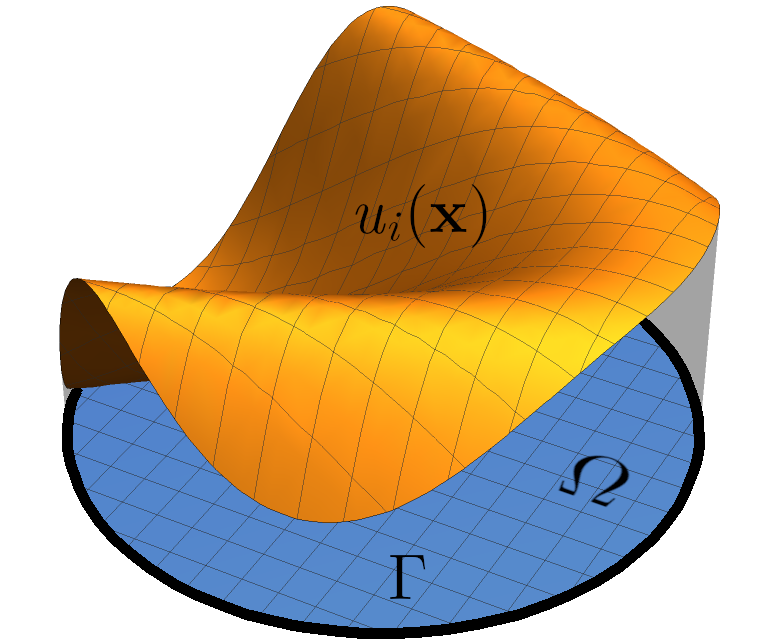
\includegraphics[width=5.5cm]{Slike/funkcijaInDomenaG}
	\caption{Domena $\Omega$, meja domene $\Gamma$ in komponenta rešitve $u_i(\mathbf{x})$.}
\label{fig:funkInDom}
\vspace{-2.6cm}
\end{wrapfigure}
Naj bo torej prizorišče dogajanja $d$-mnogoterost $\Omega$, opremljena s krajevnim vektorjem $\mathbf{x} = \{x_1, ..., x_d\}$. Pri reševanju sistema $m$ \texttt{PDE} iščemo nabor funkcij $\mathbf{u}(\mathbf{x}) =  \{u_1(\mathbf{x}), ..., u_m(\mathbf{x})\}$, ki v vsaki točki domene $\Omega$ zadosti sistemu \texttt{PDE}, na meji $\Gamma$ pa robnim pogojem (slika \ref{fig:funkInDom}). Konkretni primer bomo gradili na \textbf{sistemu Stokesovih enačb} za nestisljive tekočine v obliki \emph{u-p-$\omega$} (hitrost, tlak, vrtinčnost):\\[0.05cm]
\begin{minipage}{5.0cm}
\begin{IEEEeqnarray}{rl}
	\frac{\pd u}{\pd x} + \frac{\pd v}{\pd y} &= 0 \ , \\[0.3cm]
	\frac{\pd p}{\pd x} + \frac{\pd \omega}{\pd y} &= f_1 \ ,
\end{IEEEeqnarray}
\end{minipage}
\begin{minipage}{5.3cm}
\begin{IEEEeqnarray}{rl}
	\frac{\pd p}{\pd y} - \frac{\pd \omega}{\pd x} &= f_2 \ , \\[0.3cm]
	\omega - \frac{\pd u}{\pd y} - \frac{\pd v}{\pd x} &= 0 \ .
\end{IEEEeqnarray}
\end{minipage}\\[0.4cm]
To je le sistem stacionarnih Navier-Stokesovih enačb brez nelinearnih konvektivnih členov, ki jih moramo pri numeričnem reševanju linearizirati. Ker ta korak za ponazoritev \texttt{LSFEM} ni ključen, se mu na tak način izognemo. Kot zanimivost navržimo, da Stokesove enačbe opisujejo plazeče se tokove, pri katerih je konvekcija gibalne količine (zaradi gibanja) majhna v primerjavi z njeno difuzijo (zaradi viskoznosti). V enačbah ni časovnih odvisnosti (razen preko časovno odvisnih robnih pogojev), zato so takšni tokovi časovno obrnljivi: časovno obrnjena rešitev enačb je prav tako rešitev (slika \ref{fig:TaylorCouette}).

\begin{figure}[ht]
	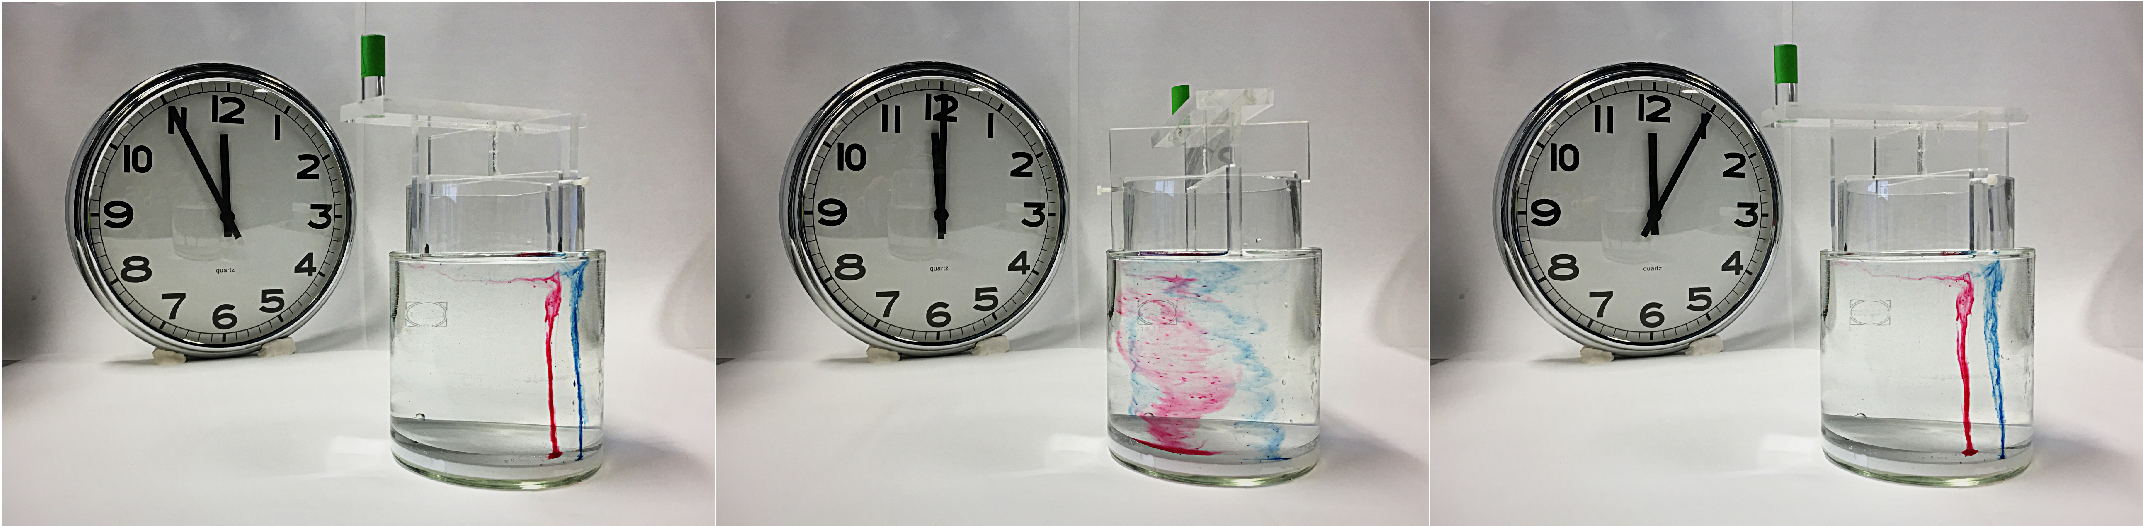
\includegraphics[width = 1\textwidth]{Slike/TaylorCouette}
	\caption{Zabaven eksperiment, pri katerem se v ozkem prostoru med dvema koncentričnima valjema nahaja viskozna tekočina, ki jo na dveh mestih označimo z liso barvila. Valja pet minut vrtimo v nasprotnih smereh (Stokesov tok, ki tako nastane, imenujemo Taylor-Couettov tok), da se lisi pomešata, nato smeri vrtenja obrnemo in po petih minutah se lisi ponovno sestavita \cite{Wiki-StokesFlow}.}
	\label{fig:TaylorCouette}
\end{figure}

Vse različice \texttt{FEM} temeljijo na variacijskem pristopu, kjer ne operiramo neposredno na \texttt{PDE}, ampak jih najprej pretvorimo v enakovreden variacijski problem: omislimo si \textbf{poskusno funkcijo} $\mathbf{w}(\mathbf{x})$, ki jo napnemo nad domeno $\Omega$, in funkcional $I[\mathbf{w}(\mathbf{x})]$, ki za vsako $\mathbf{w}(\mathbf{x})$ vrne neko realno število. Kakršenkoli funkcional pa za rešitev problema ni dober. Najti moramo takšnega, ki, ko je $\mathbf{w}(\mathbf{x})$ enaka rešitvi, vrne najmanjšo vrednost. Ponavadi je funkcional integral neke funkcije $F\left(\mathbf{w}\right)$ po domeni $\Omega$:
\begin{equation}
	I[\mathbf{w}(\mathbf{x})] = \int_{\Omega} F\left(\mathbf{w}(\mathbf{x})\right) \, \ud \Omega \hspace{1.1cm} \texttt{funkcional} \quad .
\end{equation}
Kot vemo, poiščemo minimum funkcionala $I$ tako, da za $\mathbf{w}$ vstavimo:

\setlength{\textheight}{26.5cm}			% Header Lower Margin to
\pagebreak
\setlength{\topmargin}{1.6cm}			% Header Top Margin Height
\setlength{\headheight}{0.0cm}
\setlength{\headsep}{0.0cm}			% Header Lower Margin Height	 Footer height
\fancyhf{}
\fancyfoot[C]{\thepage}
\begin{equation}
	\mathbf{w}(\mathbf{x}, \varepsilon) = \mathbf{u}(\mathbf{x}) + \varepsilon \mathbf{v}(\mathbf{x}) \quad ,
\end{equation}
kjer je $\mathbf{v}(\mathbf{x})$ poljuben odmik od rešitve $\mathbf{u}(\mathbf{x})$, $\varepsilon$ pa skalar. Odvajamo po $\varepsilon$ in odvod enačimo z 0:
\begin{equation}
\frac{\ud I}{\ud \varepsilon} = \int_{\Omega} \frac{\ud}{\ud \varepsilon} F(\mathbf{w}) \, \ud \Omega = \int_{\Omega} \frac{\ud F}{\ud \mathbf{w}} \cdot \frac{\ud \mathbf{w}}{\ud \varepsilon} \ \ud \Omega = \int_{\Omega} \frac{\ud F}{\ud \mathbf{w}} \cdot \mathbf{v} \ \ud \Omega = 0 \hspace{0.9cm} \texttt{prva variacija} \ .
\end{equation}

Fizikalno najintuitivnejša je \textbf{Rayleigh-Ritzeva različica}, kjer za $F$ uporabimo energijski potencial sistema \texttt{PDE}. Rešitev $\mathbf{u}(\mathbf{x})$ je potemtakem funkcija, ki minimizira totalno potencialno energijo sistema. Rayleigh-Ritzeva različica poseduje lastnost najboljšega približka (minimizira razliko energijskih norm numerične in eksaktne rešitve), hkrati pa vodi do sistema linearnih algebrajskih enačb, ki je zelo prikladen za reševanje s hitrimi iteracijskimi metodami.

Z Rayleigh-Ritzevo metodo dobimo sistem linearnih algebrajskih enačb za 

Galerkin, Najmanših kvadratov \cite{JiangB-LSFEM}
Basic lemma of variational principles: Temeljni lema variacijskih načel.

\textbf{Rayleigh-Ritzeva različica} \texttt{FEM}, ki je bila razvita prva in ima korenine v začetku dvajsetega stoletja (cite), je prav tako variacijska metoda.
	\appendix
	\printbibliography
\end{document}
